Thermal systems are typically characterized by macroscopic quantities, temperature, pressure, and volume, that arise from the statistical behavior of an enormous number of microscopic constituents. Each molecule in a gas possesses a definite position and velocity at every instant. Macroscopic observables summarize the collective dynamics of trillions of particles.

A single macroscopic state can correspond to an enormous number of microscopic configurations. The same pressure and temperature in a gas can arise from countless different combinations of individual molecular positions and velocities. This multiplicity is central to statistical mechanics, where a macroscopic description averages over the detailed microstates that realize it.

Entropy quantifies the logarithm of the number of microstates compatible with a given macrostate. In the Boltzmann formulation, the entropy $S$ of a system is expressed as $S = k_B \ln \Omega$, where $k_B$ is Boltzmann's constant and $\Omega$ denotes the number of microstates. This mathematical framework captures both the multiplicity of configurations and the incompleteness of macroscopic information.

The Boltzmann constant $k_B = 1.381 \times 10^{-23}$ J/K emerged from Ludwig Boltzmann's pioneering work in statistical mechanics during the late 19th century — when he sought to derive the macroscopic laws of thermodynamics from the microscopic motion of atoms and molecules. This constant serves as a bridge between the microscopic and macroscopic worlds. It converts between energy scales accessible to individual particles (measured in joules) and the thermal energy scale (measured in temperature units of kelvins). At room temperature ($T \approx 300$ K), the thermal energy $k_B T \approx 4 \times 10^{-21}$ J represents the characteristic energy of molecular motion. This tiny energy, about $0.026$ electron volts, sets the scale for thermal fluctuations, determining which molecular processes can occur spontaneously and which require external energy input. The Boltzmann constant connects the statistical behavior of countless microscopic constituents to the macroscopic thermodynamic properties we observe.

The second law of thermodynamics asserts that in an isolated system, entropy cannot decrease. Natural processes tend toward macrostates with greater multiplicity because they are overwhelmingly more probable. The law governs the irreversibility observed in macroscopic phenomena and forbids spontaneous reorganization into low-entropy configurations without intervention.


Over time, systems evolve toward equilibrium configurations through overwhelmingly probable statistical tendencies. The microscopic dynamics may allow rare fluctuations into low-entropy states. However, most accessible microstates correspond to thermal equilibrium, ensuring that systems overwhelmingly move toward higher entropy.

The second law of thermodynamics admits several equivalent formulations. In the Clausius statement, it forbids the spontaneous flow of heat from a colder body to a hotter one. In the Kelvin statement, it rules out the complete conversion of heat into mechanical work in a cyclic process without any other effect. Both formulations capture the unidirectional dispersal of energy and the impossibility of constructing perpetual motion machines of the second kind.

While the underlying microscopic laws, Newtonian mechanics or the Schrödinger equation, are time-reversal invariant, macroscopic irreversibility emerges from statistical asymmetry. Individual molecular collisions remain reversible, but the aggregate behavior overwhelmingly favors transitions toward higher-entropy macrostates due to the vast numerical dominance of such configurations.

Although the total phase space volume occupied by a system is conserved under Hamiltonian evolution, as guaranteed by Liouville's theorem, entropy can increase. Fine-grained distributions evolve into intricate structures that, when viewed with any coarse-graining appropriate to macroscopic observations, appear more uniform, corresponding to higher entropy.

Temperature reflects the average kinetic energy per degree of freedom in a system. In classical gases, the distribution of particle energies follows the Maxwell–Boltzmann distribution, while in more general statistical ensembles, the Boltzmann distribution governs the probability of finding the system in a given microstate, establishing a precise link between microscopic motion and macroscopic thermodynamic parameters.

Thermodynamic processes exchange energy between systems through work and heat, but entropy tracks the irreversible dispersal of energy and the loss of access to precise microscopic configurations. While work represents organized energy transfer and heat denotes disorganized exchange, the second law constrains their interplay, ensuring that some fraction of energy always becomes unavailable for doing work.

The second law introduces a preferred temporal direction, often termed the thermodynamic arrow of time. This arrow is not derived from the laws of motion, which are time-symmetric, but from the statistical tendency toward higher entropy. As entropy increases, systems evolve from ordered to disordered states, establishing an emergent asymmetry between past and future.

The increase of entropy is not a mechanistic necessity imposed by the microscopic equations of motion, but a near certainty based on phase space volumes. The number of microstates corresponding to high-entropy macrostates so vastly exceeds those of low-entropy macrostates that, although a reversal is technically possible, it is statistically negligible on any practical timescale.

The rise of entropy presumes a process of coarse-graining: grouping microscopic configurations that are indistinguishable at the macroscopic level. Fine-grained correlations and fluctuations, though preserved in principle by microscopic dynamics, become irrelevant for macroscopic observables, allowing entropy to increase from the observer's practical standpoint.

Entropy represents the missing information about the system's precise microstate. In this view, thermodynamic entropy parallels concepts from information theory, linking the physical evolution of systems with the epistemic limitations inherent in macroscopic descriptions.

In 1867, James Clerk Maxwell introduced a thought experiment that challenged the apparent absoluteness of the second law of thermodynamics. He imagined a sealed box filled with gas at thermal equilibrium, where molecules moved randomly at a range of speeds and directions. A partition divided the box into two chambers, A and B, with a small frictionless door controlled by a hypothetical observer: the demon.

The demon's intervention does not involve the input of mechanical work or external energy. Instead, it passively monitors individual molecules approaching the door. When a fast-moving molecule from chamber A nears the door, the demon opens it, allowing the molecule into chamber B. When a slow-moving molecule from B approaches, it is allowed into chamber A. Molecules not meeting these criteria are blocked. Over time, faster molecules accumulate in B, and slower ones in A.

\begin{center}
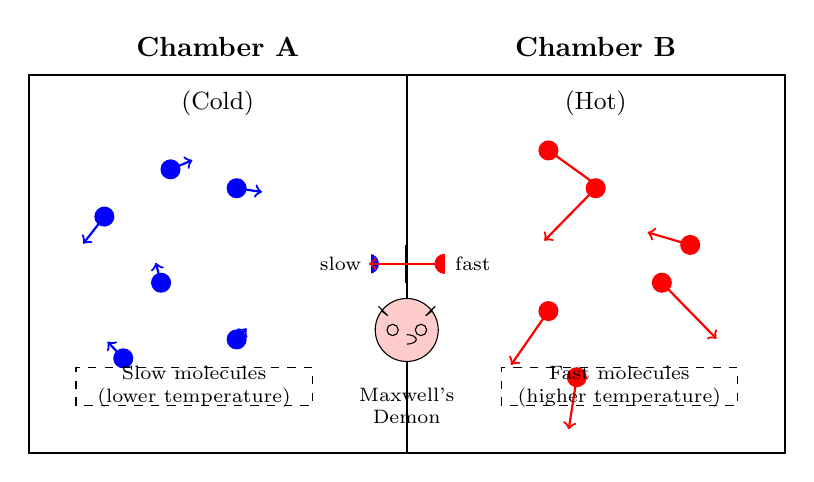
\begin{tikzpicture}[scale=1.2]
    \draw[thick] (0,0) rectangle (8,4);
    \draw[thick] (4,0) -- (4,4);
    \node[font=\bfseries] at (2,4.3) {Chamber A};
    \node[font=\bfseries] at (6,4.3) {Chamber B};
    \node[font=\small] at (2,3.7) {(Cold)};
    \node[font=\small] at (6,3.7) {(Hot)};
    \draw[very thick, fill=black!10] (4,1.8) -- (4,2.2);
    \node[draw, circle, fill=red!20, minimum size=0.8cm] (demon) at (4,1.3) {};
    \draw (demon) -- ++(0.2,0.15) -- ++(0.1,0.1);
    \draw (demon) -- ++(-0.2,0.15) -- ++(-0.1,0.1);
    \draw (demon) -- ++(0,0.4);
    \draw (demon.center) ++(0.15,0) circle (0.06);
    \draw (demon.center) ++(-0.15,0) circle (0.06);
    \draw (demon.center) ++(0,-0.15) arc (270:450:0.1 and 0.05);
    \foreach \x/\y in {1.0/1.0, 0.8/2.5, 1.5/3.0, 2.2/1.2, 2.2/2.8, 1.4/1.8}{
        \draw[thick, blue, ->] (\x,\y) -- ++({0.3*cos(rnd*360)},{0.3*sin(rnd*360)});
        \filldraw[blue] (\x,\y) circle (0.1);
    }
    \foreach \x/\y in {5.5/1.5, 6.0/2.8, 5.5/3.2, 6.7/1.8, 7.0/2.2, 5.8/0.8}{
        \draw[thick, red, ->] (\x,\y) -- ++({0.6*cos(rnd*360)},{0.6*sin(rnd*360)});
        \filldraw[red] (\x,\y) circle (0.1);
    }
    \filldraw[blue] (3.6,2.0) circle (0.1);
    \draw[->, thick, blue] (3.6,2.0) -- (4.4,2.0);
    \node[draw=white, fill=white, font=\scriptsize] at (3.3,2.0) {slow};
    \filldraw[red] (4.4,2.0) circle (0.1);
    \draw[->, thick, red] (4.4,2.0) -- (3.6,2.0);
    \node[draw=white, fill=white, font=\scriptsize] at (4.7,2.0) {fast};
    \draw[dashed] (0.5,0.5) rectangle (3.0,0.9);
    \node[align=center, font=\scriptsize] at (1.75,0.7) {Slow molecules\\(lower temperature)};
    \draw[dashed] (5.0,0.5) rectangle (7.5,0.9);
    \node[align=center, font=\scriptsize] at (6.25,0.7) {Fast molecules\\(higher temperature)};
    \node[align=center, font=\scriptsize] at (4,0.5) {Maxwell's\\Demon};
\end{tikzpicture}
\end{center}

This selective sorting induces a temperature gradient where none previously existed. Heat flows from the colder to the hotter chamber without any external energy input, in direct contradiction to the Clausius formulation of the second law. From a statistical standpoint, entropy appears to decrease: the initially uniform, high-entropy configuration is replaced by a more ordered state characterized by a temperature difference.

The paradox arises because no mechanical work is performed and no external energy is introduced, yet the system evolves toward a lower-entropy configuration. The demon, by choosing which molecules to admit or block, seems capable of circumventing the thermodynamic constraints that govern ordinary processes.

Two different approaches have emerged to resolve this paradox, each offering distinct insights into the relationship between information, work, and entropy.

\textbf{The Work-Based Approach} argues that the demon cannot operate without performing thermodynamic work. To distinguish between fast and slow molecules, the demon must interact with them, perhaps by shining light to measure their velocities or by mechanically probing their kinetic energies. These measurement processes necessarily require energy input and generate entropy. However, this approach faces a limitation: it cannot establish a precise quantitative relationship between the work invested in measurement and the entropy reduction achieved through sorting. The energy costs of individual molecular measurements depend on the specific measurement apparatus and protocols, making it difficult to prove that the entropy increase from measurement operations exactly compensates for the entropy decrease from molecular sorting.

\textbf{The Information-Erasure Approach} offers a more satisfactory resolution by focusing not on measurement costs, but on the logical requirements of cyclic operation. This approach, developed by Rolf Landauer and Charles Bennett, recognizes that for the demon to operate cyclically, it must eventually erase the information stored in its memory. Landauer's principle establishes that erasing one bit of information requires a minimum energy dissipation of $k_B T \ln 2$, where $k_B$ is Boltzmann's constant and $T$ the temperature of the environment. This energy cost is independent of the physical implementation — it represents a thermodynamic limit on information processing.

Bennett's crucial insight was that this erasure cost provides exact entropy accounting. In each cycle, the demon reduces the gas entropy by $k_B \ln 2$ (corresponding to one bit of information about molecular positions). To continue operating, the demon must erase one bit from its memory, which necessarily increases the environment's entropy by at least $k_B \ln 2$. The entropy reduction from molecular sorting is precisely compensated by the entropy increase from information erasure. No net entropy decrease occurs when all components, gas, demon memory, and thermal environment, are included in the accounting.

This information-theoretic resolution is remarkable because it establishes that \textbf{information is physical}. The demon's memory, though conceptually abstract, must be realized in some material substrate subject to thermodynamic laws. The act of erasing information is not merely a computational operation but a physical process that generates heat and increases entropy. The paradox dissolves not through appeals to measurement work or mechanical constraints — but through the thermodynamic cost of information processing.

The information-erasure approach also reveals why attempts to circumvent the erasure requirement fail. If the demon preserves information indefinitely to avoid erasure costs, its memory eventually becomes full, preventing further operation. If the demon attempts to reset its memory without erasure, perhaps through reversible computation, the information is merely transferred elsewhere in the system, requiring eventual erasure at some location. The second law cannot be circumvented by clever information management; it emerges inevitably from the statistical nature of many-body systems and the physical reality of information storage.

Recent work has further refined this picture. The "piston-demon" model suggests that the moving partition itself serves as the demon's memory, with its final position encoding information about molecular locations. Others have noted that the resolution depends crucially on how one defines the system boundaries and whether the demon-plus-gas combination constitutes a closed thermodynamic system. These discussions continue to illuminate the subtle relationships between information theory, statistical mechanics, and thermodynamic laws.

Quantum mechanics introduces additional complexities. In quantum systems, measurement necessarily disturbs the system being measured, and particles obey indistinguishability and entanglement rules that constrain sorting operations. Quantum versions of Maxwell's demon have been proposed and analyzed, demonstrating versions in which quantum coherence and decoherence affect the entropy accounting. These quantum demon studies continue to probe the connections between information, measurement, and thermodynamics at the microscopic scale.